\documentclass[12pt]{article}
\usepackage{url}
\usepackage[authoryear,round]{natbib}
\usepackage{graphicx} 

\title{Outline flowCore paper}

\author{Florian Hahne*\\
  Nolwenn LeMeur*\\
  Byron Ellis\\
  Ryan Brinkman\\
  Perry Haaland\\
  Errol Strain\\
  Deepayan Sarkar\\
  Josef Spidlen\\
  Robert Gentleman
 }

\begin{document}

\maketitle

\section*{Introduction}
Traditionally, flow cytometry (FCM) has been a tube-based technique
limited to small-scale laboratory and clinical studies.  High
throughput methods for flow cytometry (FC-HCS) have recently been
developed and are now used in both basic and clinical research. Today,
the need for flexible and well structured computational tools to
efficiently handle and analyze FC-HCS has increased
considerably. Indeed, the amount of information generated by these
technologies must be stored, managed, and needs to be summarized in
order to be accessible to the researcher. However, the absence of a
shared research platform that bioinformaticians, computer scientists,
and statisticians can utilize to develop novel or standard methods for
flow cytometric analysis has hindered innovation. We believe that the
open source statistical software R in conjunction with the
Bioconductor Project can fill this gap.  In this paper, we propose R
data structures to handle flow cytometry data through the main steps
of importing, storing, assessing and preprocessing. These structures,
along with a range of specialized methods for compensation,
transformation, gating and additional preprocessing steps, are
implemented in the newly developed Bioconductor package flowCore.  We
envision flowCore to be a solid foundation for researchers to
efficiently handle FC-HCS data and for future development of new
methods and tools for their coherent analysis.


\subsection*{R and Bioconductor}
R is a robust statistical programing environment which offers a wide
range of statistical and visualization methods developed for various
fields of application. In addition, R is an open source research
platform which bioinformaticians, computer scientists, and
statisticians routinely use to develop novel tools and methodology for
statistical data analysis. For biological applications, the
Bioconductor project has become the standard toolset
\citep{gentleman2006bos} to process data spanning a diversity of
research fields from genomics to proteomics to complex cell
biology. It is particularly geared towards the analysis of large
numeric datasets that typically arise from high throughput experiments
such as microarray gene expression analysis or FC-HCS. A shared
platform proved to be particularly beneficial for the development of
analysis routines for microarray gene expression data, and by today
many of these early innovations have been incorporated into commercial
software products, thus greatly improving the quality of gene
expression data analysis. Shared data structures have been shown to be
essential for such a collaborative effort. We envision a similar
paradigm for FC-HCS data.


\subsection*{Existing data standards and conventions}
Currently, data from flow cytometry experiments are stored in single
files following a well-defined data standard (FCS). This standard
attempts to capture much of the accompanying meta information, most of
which is produced by the measurement instrument or has to be supplied
manually by the operator upon experiment setup. However, the recent
developments in high-throughput flow cytometry are shifting the focus
of interest away from single-tube based measurements towards large and
complex experimental designs with dozens of co-variates and
influencing factors. Self-contained and self-reflective data
structures are a prerequisite to allow for coordinated analysis of
such experiments. Most of the currently available software solutions
offer only limited support for such structures, or make use of
containers like XML or binary storage formats that are designed
specifically for the mostly GUI-driven user interfaces and hence are
not easily amenable to programmatical access. In addition, the
closed-source nature of most of these products makes it impratical to
connect to and integrated the data into an analysis pipeline.

Traditionally, the majority of flow cytometry experiments have been
analyzed manually by direct data inspection in one or two dimensions,
or by very basic comparisons of summary statistics. We believe that
these approaches do not fully address the highly complex nature of FCM
data, in particular, they discard many of the fundamental aspects of
the data, such as its underlying distribution and its high-dimensional
nature. In addition, the subjective character of manual analyses are a
major obstacle to reproducibility. For FC-HCS data, unassisted manual
inspection has become way too time and labor intensive, and robust
statistical methods need to be developed to point the investigator to
the interesting aspects of the data or to potential problems. While
the expert knowledge of immunologists and researchers remains crucial
for the understanding of FCM data, we believe that tight collaboration
with other research fields such as statistics and computer science can
greatly improve the relevance of flow cytometry in today's
high-throughput paradigm.

These issues are currently being addressed by emerging new flow
cytometry data standards developed in collaboration with the ISAC Data
Standards Task Force.  The Gating-ML Candidate Recommendation (CR)
represents a proposal on how to form unambiguous XML-based gate
definitions, which can facilitate the interchange and validation of
data between different software packages with the potential of
significant increase of hardware and software interoperability. Gates
may be ordered into a hierarchical structure to describe a gating
strategy. They may be applied on parameters as in FCS files or on
transformed parameters as described by an explicit parameter
transformation. This enables the encoding of a simple analytical work
flow, in a way that allows us to reconstruct the analysis
programmatically.

The flowCore framework presented here offers import functionality for
raw data FCS files along with their complete set of file-specific meta
information (Figure~\ref{fig1:FrameWork}). Moreover, it is a software
implementations of the Gating-ML CR, which opens the possibility to
integrate flowCore in existing work flows and to communicate with
virtually every other FCM tool that adheres to the proposed
standard. In addition, the software is platform agnostic, running on
Windows, Mac OS X and Linux/Unix operating systems.

flowCore is not a GUI-driven software, and all operations are done
using a command line interface. Conceptually, it is possible to add a
more elaborate user interface on top of that, however the focus is on
a programmatic approach to enable the convenient development of novel
analysis methods. By taking the burden of data management from the
programmer and by providing well-defined APIs and a structured class
hierarchy, it is possible to readily test new ideas and to easily
extend the frameworks functionality. Both the underlying R and
Bioconductor software and flowCore itself are open source and open
development projects, thus community involvement in the developing
process is highly appreciated.



\section*{Basic data structures}
\subsection*{Flow Frame}
flowCore's primary task is the representation and basic manipulation
of flow cytometry data. This is accomplished through a data model very
close to that adopted by other Bioconductor packages used for gene
expression analysis, and thus familiar to most Bioconductor
users. Similar to any other flow tool, the basic unit of organization
in flowCore is a collection of events. We call the structure that hold
this data a flow frame. All relevant information for the collection
are stored along with the matrix of raw data values and can be
accessed programmatically. Most commonly, these are descriptors of the
stains used in the experiment and the respective measurement channels,
information about compensation performed at the instrument side and
any additional keywords the user deems to be important to annotate the
data. A number of quality checks are performed during the creation of
a flow frame to ensure data integrity. There is an extended interface
that allows for the standardized interaction with the flow data, thus
enabling the development of more specialized tools for specific tasks
of the data analysis process that all share a common API.

\subsection*{Flow Set}
In high-throughput flow cytometry, many of the analysis tasks need to
be performed consistently across multiple flow measurements, hence we
introduce the concept of a collection of flow frames called a flow
set. Flow sets store the relevant information associated with each
individual frame such as descriptions of the samples or the treatment
to which a sample was subjected, and they manage the consistent
application of operations on the individual flow frames. The burden of
keeping score of the annotation is shifted from the user to the
infrastructure, thus reducing the risk of mixups and errors that are
all too common when using more or less ad hoc spreadsheets that lack a
controlled structure. In general, there is no native ordering to a
flow set, which in a way reflects the still predominant application of
tube-based experiments rather than experiments following a
plate-design. However, the flow set structure can be readily extended
to also accommodate such spatial information \textit{(plateCore
  reference, Perry, Errol?)}.

%%Figure1 Diagram of the data structures and the basic operations
\begin{figure}
\centering
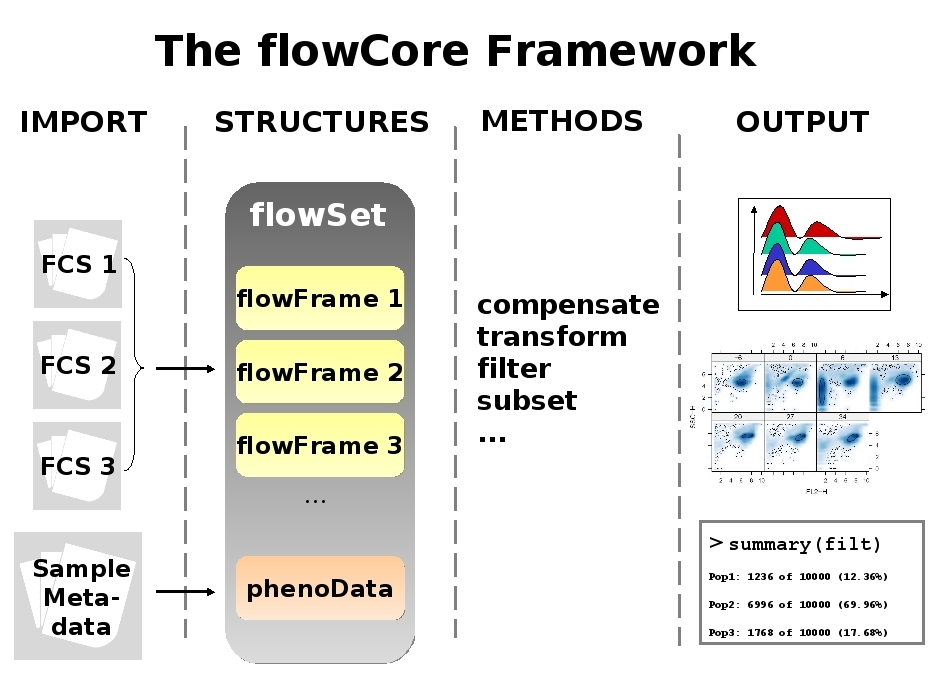
\includegraphics[width=0.9\textwidth]{Figure1-flowCoreFrameWork.jpg}
\caption{\label{fig1:FrameWork}{The flowCore frame work.For each
    experiement, FCS files, phenotypic and meta data is store in a
    flow set. Each flow frame of a flow set corresponds to one FCS
    file. All basic operation (compensation, transformation, gating,
    ...) can be applied on both single flow frames or entire flow
    set.}}
\end{figure}


\section*{Standard flow operations}
The basic operations in flow cytometry analysis are typically the
same: the data need to be compensated (if not already done on the
instrument side), often transformed and sup-population of interest
need to be selected based on a set of (predominantly sequential)
gates. All software solutions for flow data analysis offer more or
less elaborate support for these kinds of operation, most of them in
an interactive, GUI-driven spirit. The approach we have taken in
flowCore is to abstractly describe these operations and build a set of
tools to perform them on both flow frames as well as on entire flow
sets. While transformation and to a certain extent also compensation
are fairly routine operations with only limited potential for
improvement, being able to implement new methodology for gating of
flow cytometry data, and extending the capabilities of flowCore
through object oriented programming are features that clearly sets our
framework apart from other flow toolsets around. By factoring out as
much of the bookkeeping as possible, programmers can focus on the
actual operations rather then having to deal with the tedious details
of data integration and access. Third party methods implemented by
others can act on their own as first-class citizens in the analysis
framework, without breaking the workflow or the basic
infrastructure. This design allows for the straightforward extension
of flowCore's capabilities and already fostered the development of a
number of valuable improvements. \citep{lo2008agf,sarkar2008ufv}
\textit{(plateCore reference, Perry, Errol?)}.




\subsection*{Transformation and compensation}
Proper transformation have been proven beneficial for both data
visualization and modelling \citep{lo2008agf}. The major
transformations that are routinely used in flow cytometry analysis
have been implemented in flowCore. Furthermore, the design of the R
language makes it easy to define arbitrary functions to apply to the
data of individual flow frames or entire flow sets,
respectively. Compensation is available for both flow frames and flow
sets, and the software also offers functionality to compute spillover
or compensation matrices from a set of appropriate compensation
samples.



\subsection*{Gating}
In flowCore, gating operations are represented by classes that can be
extended in an object-oriented manner. Basic gate types such as
rectangular gates, ellipses and polygon gates are implemented as part
of the framework. In addition, we introduce the notion of data-driven
gates, or filters, for which the necessary parameters are computed
based on the properties of the underlying data, for instance by
modelling underlying data distribution or by density estimation. The
ability to programmatically access gates is a prerequisite for
automated or semi-automated gating. By utilizing a unified interface
for all different types of gates, the user is able to subset data sets
as well as to create summary statistics, like the proportions of
events falling in single gates or in the combinations of multiple
gates. Complex combinations and hierarchies of gates can be captured
in objects of class filterSet, allowing to apply multi-step gating
strategies. The definition of gates in flowCore follows the Gating-ML
CR, thus any flowCore gating strategy can be reproduced by any other
software that also adheres to the standard.

\section*{Related flow packages}
In addition to the flowCore package that offers basic infrastructure,
we have implemented a range of additional Bioconductor packages that
are dedicated to more specific tasks of flow cytometry data analysis
(Figure \ref{fig2:flowWheel}). The flowViz package provides
sophisticated data visualization tools, that make use of multivariate
trellis plotting. These functions can be used to quickly generate
customized plots for extended cytometry data sets for both direct data
inspection and quality control. The flowQ package offers more advanced
quality assurance (QA) methodology and a framework to create
interactive web-based reports of QA results. Most of flowUtil's
content deals with data import and output from and to flowCore and the
flow-cytometry specific standard markup languages. Finally, flowStats
provides statistical methods that are relevant in the context of flow
cytometry data analysis.


\begin{figure}
\centering
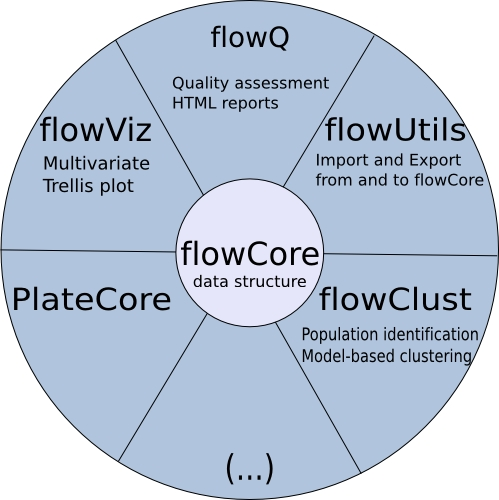
\includegraphics[width=0.6\textwidth]{Figure2-flowWheel-version4.jpg}
\caption{\label{fig2:flowWheel}{flowCore and assoziated Bioconductor
    packages: dedicated packages have been developped that utilize
    flowCore’s data structures. flowViz is a data visualization
    package; flowQ provides data quality assessment methods; flowUtils
    contains interfaces for flow data, including xml parsers:
    flowClust provides automated gating by model-based clustering.}}
\end{figure}


\section*{Application}
The flowCore package has already been applied in the analysis of a
number of datasets \citep{gasparetto2004ice,brinkman2007hcf}, and
several other Bioconductor packages are making use of its code
base. As an example, \cite{lo2008agf} have recently proposed an
automatic gating approach via robust model-based clustering using the
flowCore data model and infrastructure (implemented in the
Bioconductor package flowClust). Another package providing more
specialized support for experiments conducted on microtitre plates is
currently being developed. The documentation of all of flowCore's
features is way beyond the scope of this publication. Instead, we want
to use a single example to demonstrate some of the software's
hallmarks, that is, the concept of data-driven automated gating, the
integration of existing software into the framework and the generation
of publication-quality graphics for data visualization. The data used
for this example are flow measurements of human T-lymphocytes from 30
different patients, stained for both the CD4 and CD8 markers.

A very basic matrix of scatterplots is shown in Figure \ref{xyplot},
where each panel in the matrix represents the data of one individual
patient. Instead of plotting individual points, the local bivariate
density of the data is shown as a false color image. For each panel,
the outlines of the regions identified in the automated gating
operation described below are added to the plot. The input to the
plotting function is either a single flow frame or a complete flow set
object, and all available metadata can be accessed to control the
appearance and the composition of the plot. Similarily, gate objects
are directly passed on to the plotting function and are included in
the plot if possible. Besides the very basic scatterplot shown here,
there is a wealth of additional data visualizations available in the
flowViz package\cite{sarkar2008ufv}, all making use of flowCore's data
models allowing to easily arrange the data according to numerous
experimental factors. Furthermore, the design and the API of the
visualization software itself is very generic, and the user can
readily extend its capabilities by providing self-defined plotting
functions.

\begin{figure}[htbp]
\centering
\includegraphics[width=0.75\textwidth]{xyplot}
\caption{\label{xyplot}%
Scatterplot matrix of a single Flow Set with outlines of the gating
regions identified by an automated gating operation.}
\end{figure}

Static gating for all samples in a high-throughput flow cytometry
experiment is often not an option, since the measured variables tend
to vary between different treatments or over time. Automated or
data-driven gating tries to estimate the gating regions from the
underlying data, thus providing a fast objective solution to the
analysis of potentially very large and diverse data sets
\cite{lo2008agf}. One of the automated gating methods implemented in
flowCore is based on identifying areas of significant curvature in a
kernel density estimate of the data \citep{wand2008}. Assuming that
the regions of interest are of high density, the software is able to
reliably detect them in either the one ore the two-dimensional density
landscape. Kernel density estimation is a well-known problem in
statistical computing, and a lot of effort has been invested in the
development of good software to address it. The modular design of R,
Bioconductor and flowCore allows to easily integrate these existing
solutions into our framework. In this example, we directly use R code
from the feature package developed by Wand et al. Instead of
re-writing existing code, we are able to include it via the well
tested distribution mechanism provided by R's software package
system. This process is bi-directional, and all funtionality
implemented in flowCore is available to other package authors, as we
have seen with the afore-mentioned flowClust package.

In developing flowCore, we tried to provided a unified develoment and
analysis platform for flow-cytometry data. The scope and complexity of
the technology is evolving rapidly, and a collaborative effort in
devising new methodolgy has been proven beneficial for a number of
different biological and computational biology challenges. We hope
that our framework will be the foundation for fruitful shared research
by many calloborators from multiple scientific fields, further pushing
the boundaries of the exiting and still promising flow cytometry
technology.



\bibliographystyle{plainnat}  
\bibliography{flowCoreRef} 
\end{document}

